%%
%% Author: Antonio (yanganto@gmail.com)
%% LISENCE: CC-BY-NC
%%
\documentclass{article}        
\usepackage[a4paper,margin=0.2in,landscape]{geometry}
\usepackage{graphicx}
\usepackage{CJKutf8}


\usepackage{multicol}
\setlength{\columnsep}{13cm}


\begin{document}
\begin{CJK*}{UTF8}{bkai}
\begin{multicols}{2}

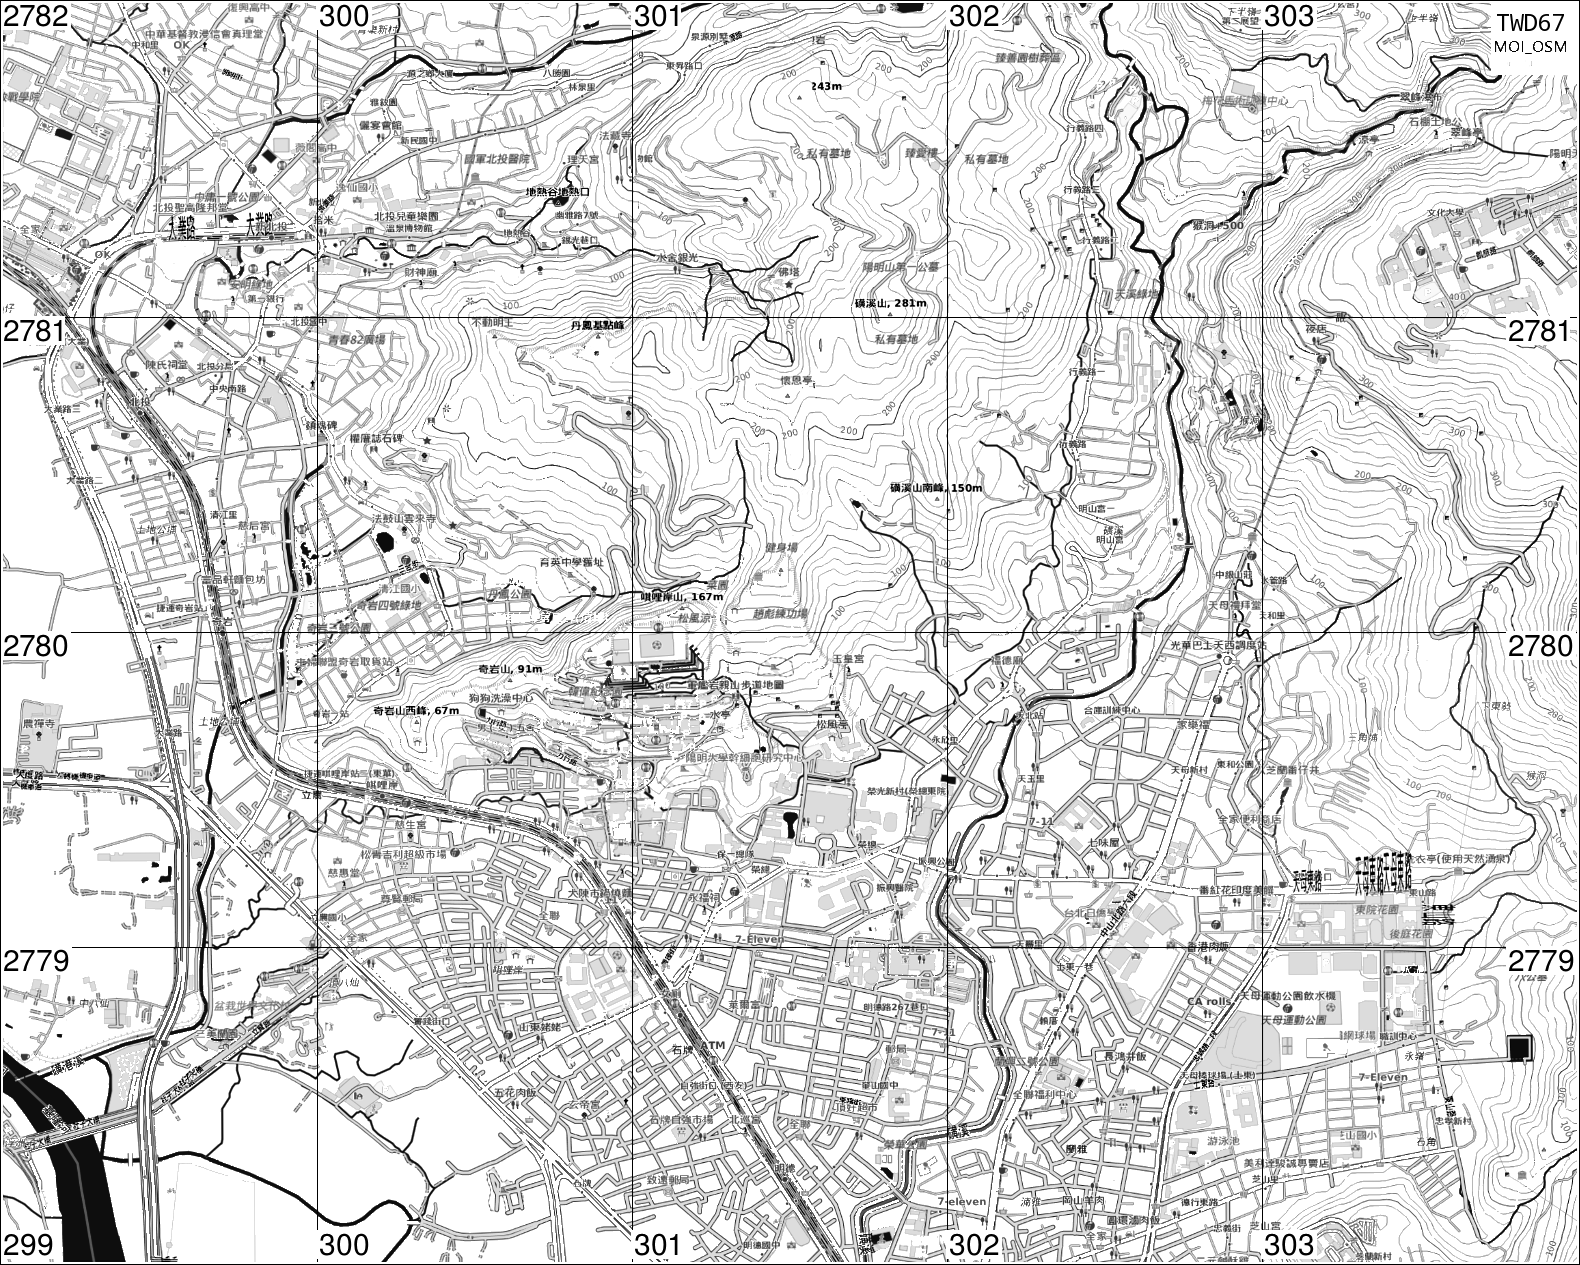
\includegraphics[width=20.73cm, height=16.58cm]{osm-map.png}

\begin{tabular}{|l|c|l|}
	\hline
	&TWD67&資訊\\  
	\hline
	\textbf{M1} 石牌&0116,7876&H8.16m\\
	\textbf{M2} 新北投&9985,8124&H16.21m\\
	\hline
	\textbf{一}\ 榮總&0136,7917&-\\
	\textbf{二}\ 陽明&0093,7927&-\\
	\textbf{三}\ 東華&0004,7956&-\\
	\textbf{四}\ 公館&9989,7966&-\\
	\textbf{五}\ 奇岩&0052,8117&-\\
	\textbf{六}\ 銀光&0083,8119&-\\
	\hline
	\textbf{A1} 變電所&0166,7974&-\\
	A2 玉皇宮& &\\
	A3 電塔& &\\
	A4 展望點& &\\
	\textbf{A5} 軍艦岩&0148,8019&C7,250$^{\circ}$GN,400m\\
	\textbf{A6} 涼亭&0155,8044&A5,200m\\
	\hline
	B1 隧道西口& &-\\
	B2 隧道東口& &-\\
	\textbf{B3} 登山口&0133,7976&-\\
	\textbf{B4} 鞍部&0127,8003&鞍部\\
	\textbf{B5} 佛字&0135,8057&兩谷夾的小稜\\
	\textbf{B6} 照明寺&0103,0870&-\\
	\hline
	C1 小廟& &-\\
	\textbf{C2} 市291&0000,7964&\\
	\textbf{C3} 奇岩西峰&0032,7970&\\
	C4 開闊地& &\\
	\textbf{C5} 奇岩山&0062,7983&\\
	C6 接馬路& &\\
	C- 圖根點&0087,7994&1654荷蘭34號\\
	\textbf{C7} 唭哩岸山&0116,8006&\\
	\hline
	D1 紀念碑& &-\\
	\textbf{D2} 市13&0041,8069&\\
	\textbf{D3} 市32&0057,8093&\\
	\textbf{D4} 水泥路底&0064,8085&\\
	\textbf{D5} 紅電塔&0085,8089&\\
	\textbf{D6} H210&0105,8090&\\
	\textbf{D7} 鞍部&0120,8077&\\
	\textbf{D8} 三叉峰&0150,8074&\\
	\hline
	\textbf{E1} 登山口&0126,8109&-\\
	E2 銀光巷底& &\\
	E3 大廣場& &\\
	E4 磺溪山& &\\
	E5 墓園高地& &\\
	E6 鐵塔& &\\
	E7 小林界碑& &\\
	E8 道路轉彎& &\\
	\hline
	\multicolumn{3}{l}{\textbf{學員僅有粗體座標}}\\
	\multicolumn{3}{l}{\textbf{A5,A6,B4,B5為範例,協助學員填空}}
\end{tabular}


\cleardoublepage

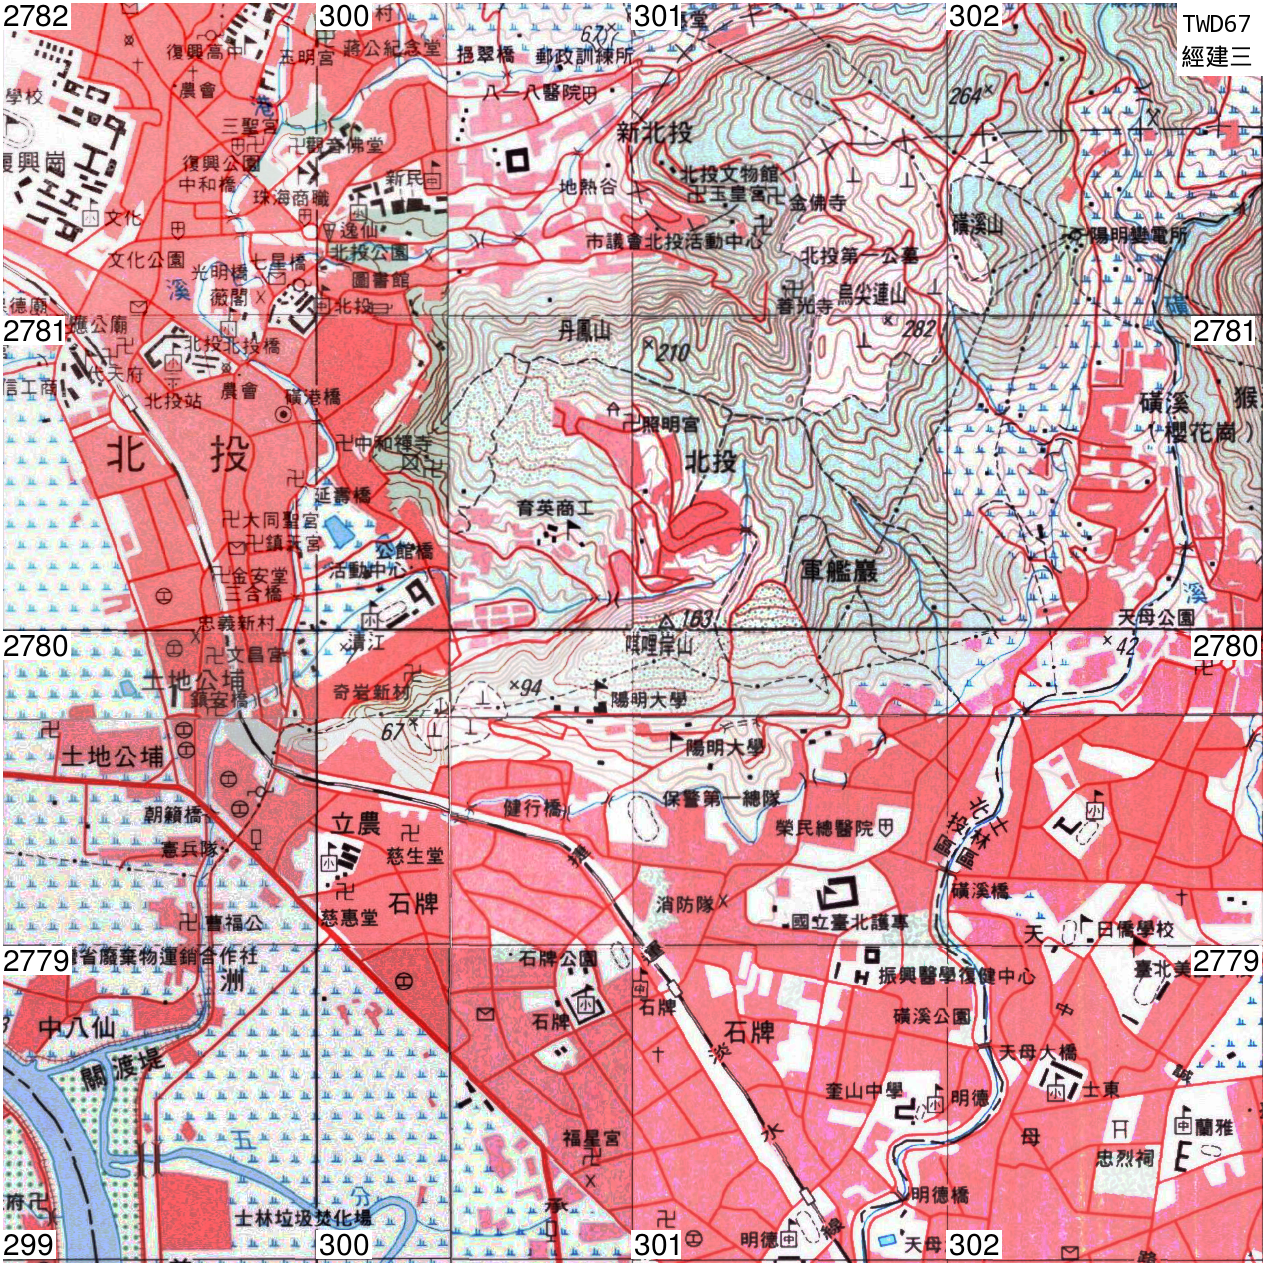
\includegraphics[width=20.73cm, height=16.58cm]{v3.png}

\begin{tabular}{|l|c|l|}
	\hline
	&TWD67&資訊\\  
	\hline
	\textbf{M1} 石牌&0116,7876&8.16m\\
	\textbf{M2} 新北投&9985,8124&16.21m\\
	\hline
	\textbf{一}\ 榮總&0136,7917&-\\
	\textbf{二}\ 陽明&0093,7927&-\\
	\textbf{三}\ 東華&0004,7956&-\\
	\textbf{四}\ 公館&9989,7966&-\\
	\textbf{五}\ 奇岩&0052,8117&-\\
	\textbf{六}\ 銀光&0083,8119&-\\
	\hline
	\textbf{A1} 變電所&0166,7974&-\\
	A2 玉皇宮& &\\
	A3 電塔& &\\
	A4 展望點& &\\
	\textbf{A5} 軍艦岩&0148,8019&C7,250$^{\circ}$GN,400m\\
	\textbf{A6} 涼亭&0155,8044&A5,200m\\
	\hline
	B1 隧道西口& &-\\
	B2 隧道東口& &-\\
	\textbf{B3} 登山口&0133,7976&-\\
	\textbf{B4} 鞍部&0127,8003&鞍部\\
	\textbf{B5} 佛字&0135,8057&兩谷夾的小稜\\
	\textbf{B6} 照明寺&0103,0870&-\\
	\hline
	C1 小廟& &-\\
	\textbf{C2} 市291&0000,7964&\\
	\textbf{C3} 奇岩西峰&0032,7970&\\
	C4 開闊地& &\\
	\textbf{C5} 奇岩山&0062,7983&\\
	C6 接馬路& &\\
	C- 圖根點&0087,7994&1654荷蘭34號\\
	\textbf{C7} 唭哩岸山&0116,8006&\\
	\hline
	D1 紀念碑& &-\\
	\textbf{D2} 市13&0041,8069&\\
	\textbf{D3} 市32&0057,8093&\\
	\textbf{D4} 水泥路底&0064,8085&\\
	\textbf{D5} 紅電塔&0085,8089&\\
	\textbf{D6} H210&0105,8090&\\
	\textbf{D7} 鞍部&0120,8077&\\
	\textbf{D8} 三叉峰&0150,8074&\\
	\hline
	\textbf{E1} 登山口&0126,8109&-\\
	E2 銀光巷底& &\\
	E3 大廣場& &\\
	E4 磺溪山& &\\
	E5 墓園高地& &\\
	E6 鐵塔& &\\
	E7 小林界碑& &\\
	E8 道路轉彎& &\\
	\hline
	\multicolumn{3}{l}{\textbf{學員僅有粗體座標}}\\
	\multicolumn{3}{l}{\textbf{A5,A6,B4,B5為範例,協助學員填空}}
\end{tabular}
\end{multicols}
\end{CJK*}

\end{document}

